\chapter{Architecture Constraints}

\section{Environment}
\label{sec:Environment}

\begin{longtable}{|l|l|l|}
\hline
\begin{minipage}{0.14\linewidth}\raggedright\vspace{.75ex}\textbf{Tool Name}\vspace{.75ex}\end{minipage} & \begin{minipage}{0.14\linewidth}\raggedright\vspace{.75ex}\textbf{Version}\vspace{.75ex}\end{minipage} & \begin{minipage}{0.64\linewidth}\raggedright\vspace{.75ex}\textbf{Description}\vspace{.75ex}\end{minipage}\\
\hline\hline
\endfirsthead
\hline
\begin{minipage}{0.14\linewidth}\raggedright\vspace{.75ex}\textbf{Tool Name}\vspace{.75ex}\end{minipage} & \begin{minipage}{0.14\linewidth}\raggedright\vspace{.75ex}\textbf{Version}\vspace{.75ex}\end{minipage} & \begin{minipage}{0.64\linewidth}\raggedright\vspace{.75ex}\textbf{Description}\vspace{.75ex}\end{minipage}\\
\hline\hline
\endhead
\hline
\endfoot
\hline
\endlastfoot
\begin{minipage}{0.14\linewidth}\raggedright\vspace{.75ex}ISOLAR-AB\vspace{.75ex}\end{minipage} & \begin{minipage}{0.14\linewidth}\raggedright\vspace{.75ex}12.3.3BETA1\vspace{.75ex}\end{minipage} & \begin{minipage}{0.64\linewidth}\raggedright\vspace{.75ex}AUTOSAR Authoring and BSW Configuration tools.\vspace{.75ex}\end{minipage}\\\hline
\begin{minipage}{0.14\linewidth}\raggedright\vspace{.75ex}RTA-BSW\vspace{.75ex}\end{minipage} & \begin{minipage}{0.14\linewidth}\raggedright\vspace{.75ex}12.3.3pr1\vspace{.75ex}\end{minipage} & \begin{minipage}{0.64\linewidth}\raggedright\vspace{.75ex}BSW automatic configuration and code generation.\vspace{.75ex}\end{minipage}\\\hline
\begin{minipage}{0.14\linewidth}\raggedright\vspace{.75ex}RTA-RTE\vspace{.75ex}\end{minipage} & \begin{minipage}{0.14\linewidth}\raggedright\vspace{.75ex}12.4.0\vspace{.75ex}\end{minipage} & \begin{minipage}{0.64\linewidth}\raggedright\vspace{.75ex}RTE generator used for testing.\vspace{.75ex}\end{minipage}\\\hline
\begin{minipage}{0.14\linewidth}\raggedright\vspace{.75ex}MemMapGen\vspace{.75ex}\end{minipage} & \begin{minipage}{0.14\linewidth}\raggedright\vspace{.75ex}12.3.0\vspace{.75ex}\end{minipage} & \begin{minipage}{0.64\linewidth}\raggedright\vspace{.75ex}Memory Map file generator.\vspace{.75ex}\end{minipage}\\\hline
\begin{minipage}{0.14\linewidth}\raggedright\vspace{.75ex}CANTATA\vspace{.75ex}\end{minipage} & \begin{minipage}{0.14\linewidth}\raggedright\vspace{.75ex}9.5\vspace{.75ex}\end{minipage} & \begin{minipage}{0.64\linewidth}\raggedright\vspace{.75ex}Used for functional testing.\vspace{.75ex}\end{minipage}\\\hline
\end{longtable}

\section{Layers Definition}

\begin{center}
	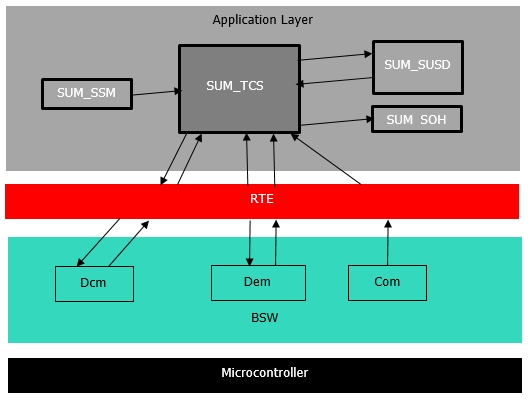
\includegraphics{images/layers.png}
\end{center}

The applied system architecture is based on Autosar v4.0.3. For detailed information on it refer to Autosar.org website.

\section{Generic component interface}
\label{sec:Generic_Component_Interface}

\UMLDiagramModified{generated/diagrams/Generic_Component_Interface}{Generic Component Interface}{0.5}

\subsection{Port Interfaces}
\label{sec:port-interfaces}

\Requirement{023}
{\begin{longtable}{|l|l|l|l|l|}
\hline
\begin{minipage}{0.32\linewidth}\raggedright\vspace{.75ex}\textbf{Port Interface}\vspace{.75ex}\end{minipage} & \begin{minipage}{0.11\linewidth}\raggedright\vspace{.75ex}\textbf{Port Type}\vspace{.75ex}\end{minipage} & \begin{minipage}{0.11\linewidth}\raggedright\vspace{.75ex}\textbf{P-Port}\vspace{.75ex}\end{minipage} & \begin{minipage}{0.11\linewidth}\raggedright\vspace{.75ex}\textbf{R-Port}\vspace{.75ex}\end{minipage} & \begin{minipage}{0.21\linewidth}\raggedright\vspace{.75ex}\textbf{Description}\vspace{.75ex}\end{minipage}\\
\hline\hline
\endfirsthead
\hline
\begin{minipage}{0.32\linewidth}\raggedright\vspace{.75ex}\textbf{Port Interface}\vspace{.75ex}\end{minipage} & \begin{minipage}{0.11\linewidth}\raggedright\vspace{.75ex}\textbf{Port Type}\vspace{.75ex}\end{minipage} & \begin{minipage}{0.11\linewidth}\raggedright\vspace{.75ex}\textbf{P-Port}\vspace{.75ex}\end{minipage} & \begin{minipage}{0.11\linewidth}\raggedright\vspace{.75ex}\textbf{R-Port}\vspace{.75ex}\end{minipage} & \begin{minipage}{0.21\linewidth}\raggedright\vspace{.75ex}\textbf{Description}\vspace{.75ex}\end{minipage}\\
\hline\hline
\endhead
\hline
\endfoot
\hline
\endlastfoot
\begin{minipage}{0.32\linewidth}\raggedright\vspace{.75ex}TCS\_SWC\_Clock\vspace{.75ex}\end{minipage} & \begin{minipage}{0.11\linewidth}\raggedright\vspace{.75ex}Sender / Receiver\vspace{.75ex}\end{minipage} & \begin{minipage}{0.11\linewidth}\raggedright\vspace{.75ex}SUM\_TCS\vspace{.75ex}\end{minipage} & \begin{minipage}{0.11\linewidth}\raggedright\vspace{.75ex}SUM\_SOH\vspace{.75ex}\end{minipage} & \begin{minipage}{0.21\linewidth}\raggedright\vspace{.75ex}Provides timestamp data for error monitoring.\vspace{.75ex}\end{minipage}\\\hline
\begin{minipage}{0.32\linewidth}\raggedright\vspace{.75ex}TimeSyncMessage\vspace{.75ex}\end{minipage} & \begin{minipage}{0.11\linewidth}\raggedright\vspace{.75ex}Sender / Receiver\vspace{.75ex}\end{minipage} & \begin{minipage}{0.11\linewidth}\raggedright\vspace{.75ex}remote SW-C\vspace{.75ex}\end{minipage} & \begin{minipage}{0.11\linewidth}\raggedright\vspace{.75ex}SUM\_TCS\vspace{.75ex}\end{minipage} & \begin{minipage}{0.21\linewidth}\raggedright\vspace{.75ex}Master Clock Signal received from TS\_Master ECU.\vspace{.75ex}\end{minipage}\\\hline
\begin{minipage}{0.32\linewidth}\raggedright\vspace{.75ex}TimeSyncMessage\_Av\vspace{.75ex}\end{minipage} & \begin{minipage}{0.11\linewidth}\raggedright\vspace{.75ex}Sender / Receiver\vspace{.75ex}\end{minipage} & \begin{minipage}{0.11\linewidth}\raggedright\vspace{.75ex}SUM\_SSM\vspace{.75ex}\end{minipage} & \begin{minipage}{0.11\linewidth}\raggedright\vspace{.75ex}SUM\_TCS\vspace{.75ex}\end{minipage} & \begin{minipage}{0.21\linewidth}\raggedright\vspace{.75ex}Availability of the Master Clock Signal.\vspace{.75ex}\end{minipage}\\\hline
\begin{minipage}{0.32\linewidth}\raggedright\vspace{.75ex}SUSD\_TCS\_PermitExecution\vspace{.75ex}\end{minipage} & \begin{minipage}{0.11\linewidth}\raggedright\vspace{.75ex}Sender / Receiver\vspace{.75ex}\end{minipage} & \begin{minipage}{0.11\linewidth}\raggedright\vspace{.75ex}SUM\_SUSD\vspace{.75ex}\end{minipage} & \begin{minipage}{0.11\linewidth}\raggedright\vspace{.75ex}SUM\_TCS\vspace{.75ex}\end{minipage} & \begin{minipage}{0.21\linewidth}\raggedright\vspace{.75ex}Informs SUM\_TCS whether it is allowed to perform its functions.\vspace{.75ex}\end{minipage}\\\hline
\begin{minipage}{0.32\linewidth}\raggedright\vspace{.75ex}TCS\_SUSD\_ShutdownPermission\vspace{.75ex}\end{minipage} & \begin{minipage}{0.11\linewidth}\raggedright\vspace{.75ex}Sender / Receiver\vspace{.75ex}\end{minipage} & \begin{minipage}{0.11\linewidth}\raggedright\vspace{.75ex}SUM\_TCS\vspace{.75ex}\end{minipage} & \begin{minipage}{0.11\linewidth}\raggedright\vspace{.75ex}SUM\_SUSD\vspace{.75ex}\end{minipage} & \begin{minipage}{0.21\linewidth}\raggedright\vspace{.75ex}Informs SUM\_SUSD whether SUM\_TCS is ready for a shutdown.\vspace{.75ex}\end{minipage}\\\hline
\begin{minipage}{0.32\linewidth}\raggedright\vspace{.75ex}TCS\_Dem\_Clock\vspace{.75ex}\end{minipage} & \begin{minipage}{0.11\linewidth}\raggedright\vspace{.75ex}Client / Server\vspace{.75ex}\end{minipage} & \begin{minipage}{0.11\linewidth}\raggedright\vspace{.75ex}SUM\_TCS\vspace{.75ex}\end{minipage} & \begin{minipage}{0.11\linewidth}\raggedright\vspace{.75ex}Dem\vspace{.75ex}\end{minipage} & \begin{minipage}{0.21\linewidth}\raggedright\vspace{.75ex}Provides Dem with timestamp data to write in the extended data record of a DTC.\vspace{.75ex}\end{minipage}\\\hline
\begin{minipage}{0.32\linewidth}\raggedright\vspace{.75ex}TCS\_Dcm\_Clock\vspace{.75ex}\end{minipage} & \begin{minipage}{0.11\linewidth}\raggedright\vspace{.75ex}Client / Server\vspace{.75ex}\end{minipage} & \begin{minipage}{0.11\linewidth}\raggedright\vspace{.75ex}SUM\_TCS\vspace{.75ex}\end{minipage} & \begin{minipage}{0.11\linewidth}\raggedright\vspace{.75ex}Dcm\vspace{.75ex}\end{minipage} & \begin{minipage}{0.21\linewidth}\raggedright\vspace{.75ex}Used to implement the Read function of DID F129.\vspace{.75ex}\end{minipage}\\\hline
\begin{minipage}{0.32\linewidth}\raggedright\vspace{.75ex}RP\_NvMService\_TCSTimeValue\vspace{.75ex}\end{minipage} & \begin{minipage}{0.11\linewidth}\raggedright\vspace{.75ex}Client / Server\vspace{.75ex}\end{minipage} & \begin{minipage}{0.11\linewidth}\raggedright\vspace{.75ex}NVM\vspace{.75ex}\end{minipage} & \begin{minipage}{0.11\linewidth}\raggedright\vspace{.75ex}SUM\_TCS\vspace{.75ex}\end{minipage} & \begin{minipage}{0.21\linewidth}\raggedright\vspace{.75ex}Needed to use NVM services to store \code{SumTCSInitValue}.\vspace{.75ex}\end{minipage}\\\hline
\begin{minipage}{0.32\linewidth}\raggedright\vspace{.75ex}RP\_SUSD\_TCS\_BatteryVoltage\_ DisableNVMWrite\vspace{.75ex}\end{minipage} & \begin{minipage}{0.11\linewidth}\raggedright\vspace{.75ex}Sender / Receiver\vspace{.75ex}\end{minipage} & \begin{minipage}{0.11\linewidth}\raggedright\vspace{.75ex}SUM\_SUSD\vspace{.75ex}\end{minipage} & \begin{minipage}{0.11\linewidth}\raggedright\vspace{.75ex}SUM\_TCS\vspace{.75ex}\end{minipage} & \begin{minipage}{0.21\linewidth}\raggedright\vspace{.75ex}Needed to read battery voltage condition to perform NvmWrite.\vspace{.75ex}\end{minipage}\\\hline
\end{longtable}}
{\Satisfies{SRS_TCS 009} \Satisfies{SRS_TCS 012}  \Satisfies{SRS_TCS 018} \Satisfies{SRS_TCS 031}}

\subsection{TCS DID services to Dcm}
\label{sec:DID}

\Requirement{025}
{\begin{longtable}{|l|l|l|l|l|l|}
\hline
\begin{minipage}{0.09\linewidth}\raggedright\vspace{.75ex}\textbf{DID Name}\vspace{.75ex}\end{minipage} & \begin{minipage}{0.09\linewidth}\raggedright\vspace{.75ex}\textbf{ID}\vspace{.75ex}\end{minipage} & \begin{minipage}{0.22\linewidth}\raggedright\vspace{.75ex}\textbf{Range}\vspace{.75ex}\end{minipage} & \begin{minipage}{0.09\linewidth}\raggedright\vspace{.75ex}\textbf{Access}\vspace{.75ex}\end{minipage} & \begin{minipage}{0.09\linewidth}\raggedright\vspace{.75ex}\textbf{Default Value}\vspace{.75ex}\end{minipage} & \begin{minipage}{0.26\linewidth}\raggedright\vspace{.75ex}\textbf{Description}\vspace{.75ex}\end{minipage}\\
\hline\hline
\endfirsthead
\hline
\begin{minipage}{0.09\linewidth}\raggedright\vspace{.75ex}\textbf{DID Name}\vspace{.75ex}\end{minipage} & \begin{minipage}{0.09\linewidth}\raggedright\vspace{.75ex}\textbf{ID}\vspace{.75ex}\end{minipage} & \begin{minipage}{0.22\linewidth}\raggedright\vspace{.75ex}\textbf{Range}\vspace{.75ex}\end{minipage} & \begin{minipage}{0.09\linewidth}\raggedright\vspace{.75ex}\textbf{Access}\vspace{.75ex}\end{minipage} & \begin{minipage}{0.09\linewidth}\raggedright\vspace{.75ex}\textbf{Default Value}\vspace{.75ex}\end{minipage} & \begin{minipage}{0.26\linewidth}\raggedright\vspace{.75ex}\textbf{Description}\vspace{.75ex}\end{minipage}\\
\hline\hline
\endhead
\hline
\endfoot
\hline
\endlastfoot
\begin{minipage}{0.09\linewidth}\raggedright\vspace{.75ex}Total Vehicle Time Value\vspace{.75ex}\end{minipage} & \begin{minipage}{0.09\linewidth}\raggedright\vspace{.75ex}0xF129\vspace{.75ex}\end{minipage} & \begin{minipage}{0.22\linewidth}\raggedright\vspace{.75ex}0 - 1,099,511,627,775 ms\vspace{.75ex}\end{minipage} & \begin{minipage}{0.09\linewidth}\raggedright\vspace{.75ex}Read\vspace{.75ex}\end{minipage} & \begin{minipage}{0.09\linewidth}\raggedright\vspace{.75ex}0 ms\vspace{.75ex}\end{minipage} & \begin{minipage}{0.26\linewidth}\raggedright\vspace{.75ex}Total Vehicle Time Value is a running time counter that is received by the Time Leader. This counter is locally incremented by Time Followers, when the signal is not available, and is also used for Time Stamping.\vspace{.75ex}\end{minipage}\\\hline
\end{longtable}}
{\Satisfies{SRS_TCS 024} \Satisfies{SRS_TCS 025}}

\section{Other constraints and assumptions}

\subsection{Assumptions}
\label{sec:assumptions}

\begin{enumerate}
\item The common interfaces among SUMs and SWCs are defined in \file{GM_SUM_Interfaces.arxml}.
\item The ports and interfaces unique to SUM_TCS shall be provided in \file{SUM_TCS_Cfg_SWCD.arxml}.
\item The resolution of a \code{TimeSyncMessage} is 100 ms.
This is equal to saying that the timestamp in the \code{TimeSyncMessage} is a counter representing the number of 100 ms increments.
It follows that the 36 bits of the \code{TimeSyncMessage} can represent up to $2^{36} \cdot 100$ ms (approximately 6.872E9 seconds, 79536 days, 217 years).
\end{enumerate}

\subsection{Constraints}
\label{sec:constraints}

\begin{description}
\item[Internal Data Types:] Special design considerations have been taken into account due to the configurability required to implement SUM_TCS.
Data types which are not defined exclusively in the RTE are used in order to facilitate the configuration required for this module.
\item[Non-Volatile Memory Access:] In order to fulfill the requirement to store the \code{SumTCSInitValue} in memory, a RAM mirror block is used for storing this data in non-volatile memory.
It is assumed the user will configure the NVM stack to support this required information.
Further, it is expected that during shutdown, the appropriate BSW services will write that specific NVM block to persistent storage. The operation should be performed only if the battery voltage is good after checking it from SUM_SUSD.
\item[Exlusive Areas:] In order to prohibit concurrent data access, SUM_TCS configures each runnable to use the \code{RunsInsideExclusiveArea} protection.
\end{description}